\section{Problem Specification}
This protocol determines the negotiation taking place between a buyer and a seller. The outcome of the protocol might be as follows:
\begin{enumerate}
\item The two parties agree on a final agreement by which the seller sells a certain quantity
of a certain product to the buyer at a certain price. Note that the product, the
quantity, and the price are all abstracted here as an INFO exchanged between the
participants;
\item the two parties might end up by not succeeding in finding an agreement;
\end{enumerate}

\begin{figure}
\centering
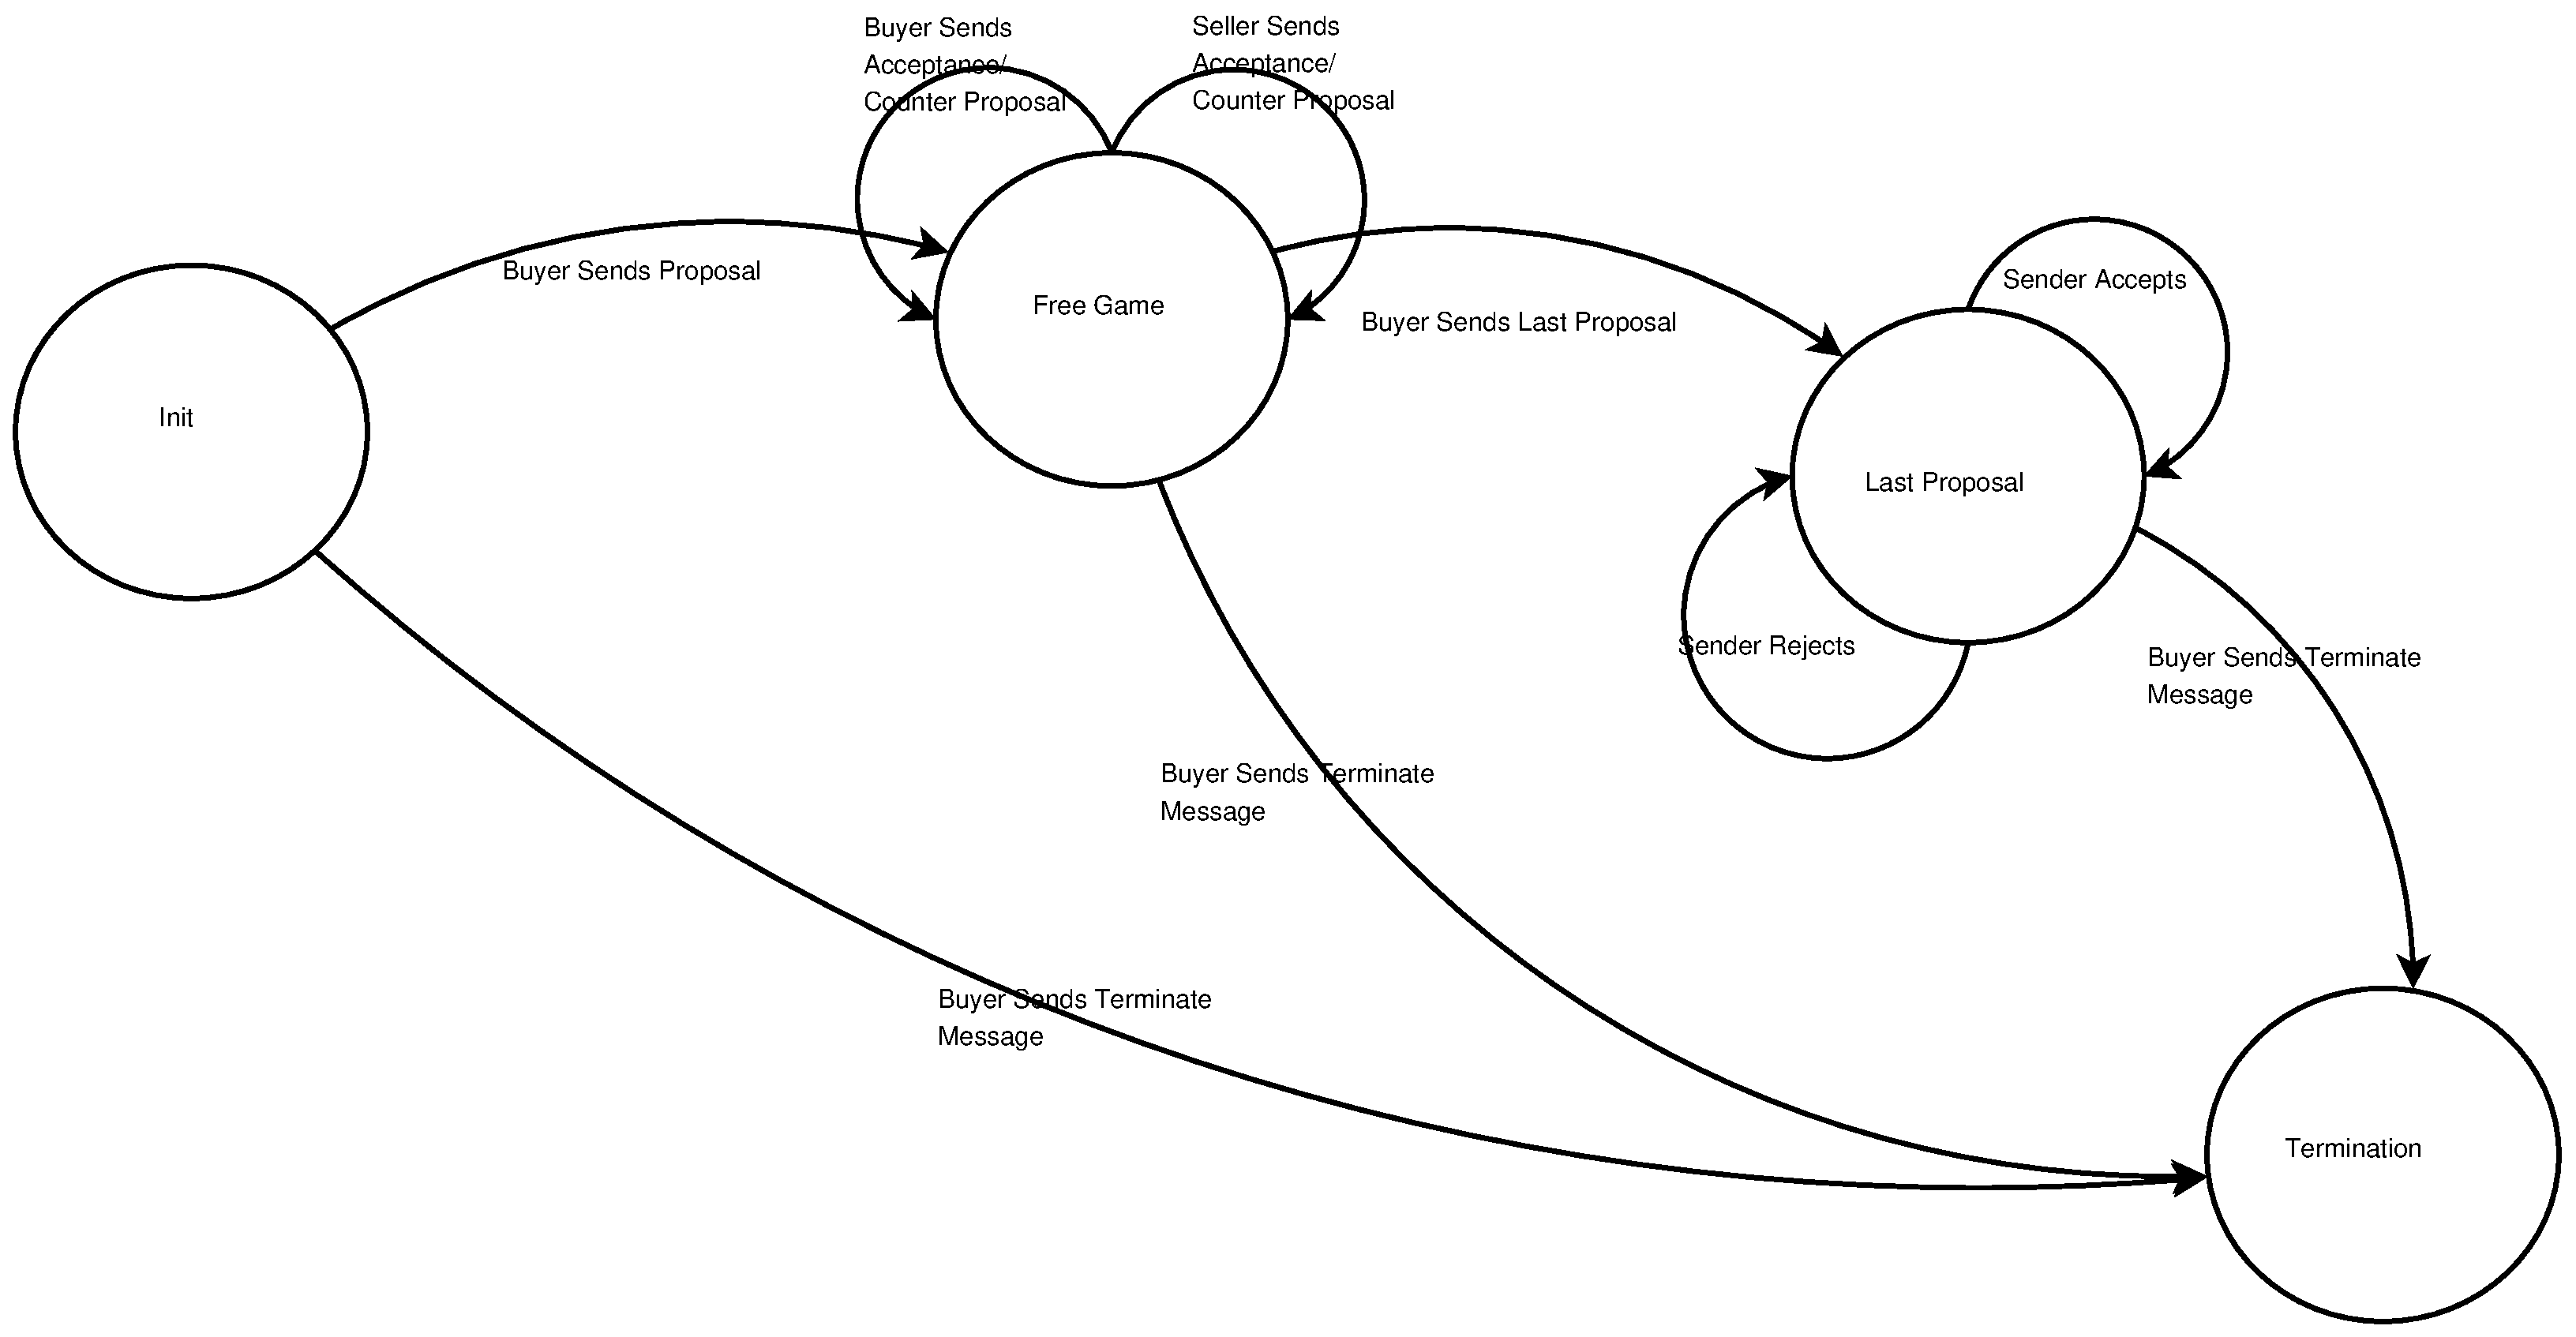
\epsfig{file=FSM.eps, width=6in}
\caption{State Transition Diagram}
\label{statetransitions}
\end{figure}

The protocol is divided into four phases: the \emph{initial} phase, the \emph{free game phase}, the \emph{last proposal} phase, and the \emph{termination} phase. (Refer Figure \ref{statetransitions}). 

\begin{itemize}
\item In the initial phase, the buyer starts the protocol by sending a proposal to the seller, which the seller must acknowledge
\item After this initial proposal has been received by the seller, and the Ack has been received by the buyer, the protocol enters the free game phase. In this second phase buyer and seller can send counter-proposal or acceptance to the other partner proposal in a fully asynchronous way. In this phase, an acceptance or a counter-proposal by either party is never definitive. We abstract the acceptance/counter proposal as just Data, which the buyer and seller may send and receive asynchronously.
\item The last proposal phase is at the initiative of the buyer which makes it clear to the seller that the proposal sent to it is the last one; the seller can either accept it or reject it. It cannot send a counter-proposal. In our model, the seller does this by the Ack message itself.
\item The termination phase is reached after the buyer sends a termination message, which the seller has to acknowledge. The termination phase can be broken into two states - the \emph{success} state and the \emph{failure} state. The \emph{end} event is an observer, that can only be called in the termination state.
\end{itemize}

During the three first phases, the buyer can always cancel the protocol by sending a
\emph{fail} message to the seller, which needs to acknowledge it. This has the immediate effect to
move the protocol to the failure phase. When in the free game state, the buyer may choose
to send a \emph{succeed} message, which causes the protocol to move to the success state.

The channels between the buyer and seller are assumed to be reliable, so that messages sent are
guaranteed to be delivered to the intended recipient.
